\chapter{Evaluation of the implementation's overhead}
\label{chapter:evaluation}

\section{RAM}
\label{sec:evaluation:ram_overhead}

\subsection{Heap}

The \nameref{sec:design:riot_registry} does not do any dynamic heap allocations, so evaluating the heap overhead is not necessary.

\subsection{Stack}

In this section the stack consumption of the \nameref{sec:design:riot_registry} \gls{ac:api} is measured and discussed.
More specifically the functions ``registry\_get\_value'', registry\_set\_value, ``registry\_commit'', ``registry\_export'', ``registry\_save'' and ``registry\_load'' are measured.

\subsubsection{Method}

To measure the stack usage of a function in \gls{gl:riot_os} is possible, because the stack implementation internally marks parts of the stack that have been ``touched''.
This way the highest ever used stack count can be printed out, but this also has the downside that before starting the measurement, the currently highest measured stack count must be equal to the current stack count.
This can be achieved by creating a new thread, which start stack count is equal to the highest stack count until that moment.

This leads to the following stack consumption measurement strategy:
\begin{enumerate}
    \item Create a new thread.
    \item Get the current stack count (highest).
    \item Save the current stack count to a variable.
    \item Call the function which stack consumption needs to be measured.
    \item Get the highest stack count.
    \item Subtract the old stack count from the new stack count.
    \item Print out the result to the terminal.
\end{enumerate}

\subsubsection{Measurements}

\autoref{table:stack_overhead} and \autoref{fig:evaluation:stack_overhead_chart} show the result of this measurement in bytes.
The first row of \autoref{table:stack_overhead} tells the length of the \gls{ac:cp}, all following rows show the stack consumption of each function per \gls{ac:cp} length.
The result shows that almost all functions don't increase their overall stack consumption at all if the \gls{ac:cp} length changes.
One exception is ``registry\_export'', which has a increase of 16 bytes (+1.5\%) from a \gls{ac:cp} with the length of 1 to a \gls{ac:cp} with the length of 2 and it also has another increase of 16 bytes from a \gls{ac:cp} with the length of 4 to a \gls{ac:cp} with the length of 5.
The other exception is the function ``registry\_save'', which oscillates between a stack consumption of up to 3,900 and down to 3,340.

\begin{table}[H]
    \begin{tabular}{ | l | r | r | r | r | r | }
        \hline
        Function \textbackslash{ \gls{ac:cp} length} & 1     & 2     & 3     & 4     & 5
        \\ \hline
        registry\_get\_value                         & 276   & 276   & 276   & 276   & 276   \\ \hline
        registry\_set\_value                         & 308   & 308   & 308   & 308   & 308   \\ \hline
        registry\_commit                             & 464   & 464   & 464   & 464   & 464   \\ \hline
        registry\_export                             & 1,092 & 1,108 & 1,108 & 1,108 & 1,124 \\ \hline
        registry\_save                               & 3,884 & 3,340 & 3,900 & 3,340 & 3,356 \\ \hline
        registry\_load                               & 2,636 & 2,636 & 2,636 & 2,636 & 2,636 \\ \hline
    \end{tabular}
    \caption{Stack consumption of \nameref{sec:design:riot_registry} \gls{ac:api} functions in bytes.}
    \label{table:stack_overhead}
\end{table}

\autoref{fig:evaluation:stack_overhead_chart} shows the stack consumption of each main \nameref{sec:design:riot_registry} function on the y axis in bytes.
The x axis shows the length of the \gls{ac:cp} that was passed to each function.

\begin{figure}[H]
    \centering
    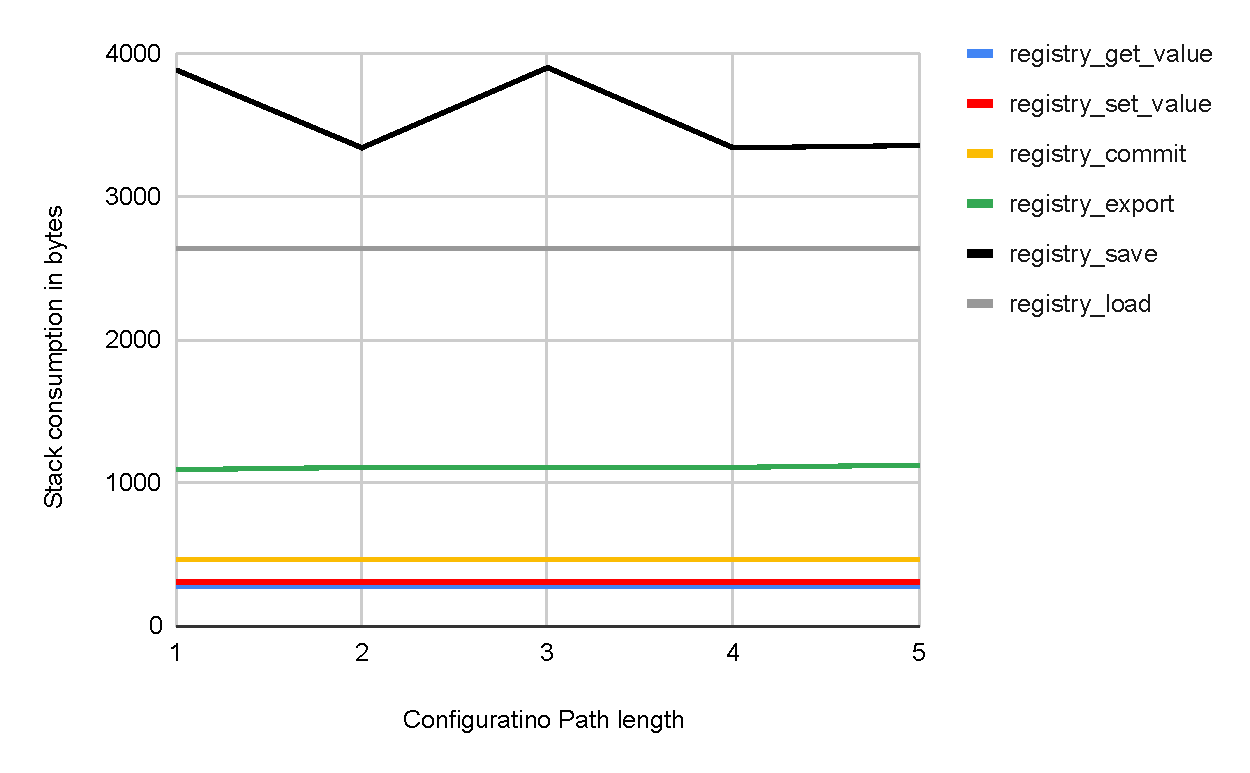
\includegraphics[width=\textwidth]{evaluation_stack_consumption_chart}
    \caption{\nameref{sec:design:riot_registry} stack consumption in bytes per \gls{ac:api} function on the \gls{ac:cp} lengths 0 - 5.}
    \label{fig:evaluation:stack_overhead_chart}
\end{figure}

\subsubsection{Discussion}

Overall the results of these measurements are not unexpected and possible to explain.
The ``set'' and ``get'' function are implemented without recursion and should not consume more stack only because they need to go deeper into the \gls{ac:cs} structure.
The ``commit'' function has a similar implementation to the ``get'' and ``set'' functions, but still consumes more stack because its slightly more complex implementation is currently distributed among multiple functions that call each other and it also needs to call the callback function of the \gls{ac:si} to inform the driver / module about the to be applied changes (see \autoref{fig:behavioral_flow_of_the_commit_api} and \autoref{fig:behavioral_flow_of_the_set_api} for comparison).
The ``export'' function is similar implemented to the ``commit'' function (see \autoref{fig:behavioral_flow_of_the_export_api}) and has its logic distributed among multiple functions, that call each other.
The major difference, that also causes the much higher stack usage is that each of these functions take up to 7 times more arguments.

The stack consumption of the ``registry\_save'' and ``registry\_load'' functions however  are more difficult to discuss.
In this example both use a \gls{ac:sf} that internally uses the \gls{gl:riot_os} \gls{ac:vfs} layer, which abstracts over filesystems such as FatFs or littlefs.
In this case the littlefs abstraction is used.
What happens with littlefs internally is unknown, but the measurements behave reasonable in contrast to how the \gls{ac:vfs} \gls{ac:sf} is implemented.
Both functions do not use recursive function calls and only rely on while loops that reuse data structures.
As a consequence also these two function don not consume more stack in relation to the \gls{ac:cp} length.
But this conclusion is only valid for the \gls{ac:vfs} \gls{ac:sf}.
Other implementations may show different results.

In general the implementation of all the analyzed functions can be improved.
Especially the distribution into multiple functions that call each other by passing on a lot of arguments is not ideal.
It makes the source code less difficult to maintain, but has the consequence of consuming unnecessarily much stack.
It should theoretically be possible to make the functions ``get'', ``set'', ``commit'' and ``export'' consume almost the same amount of stack with a more better implementation.
Of course there would still be some differences caused by the different requirements of these functions. Such things as the callback of the ``commit'' function.

\section{ROM}
\label{sec:evaluation:rom_overhead}

\gls{gl:riot_os} has a tool called ``Cosy''.
It can be used as a build target and analyzes the last build binary size in different categories.
To compare the ROM size of a \gls{gl:riot_os} application with and without the \nameref{sec:design:riot_registry}, the application is analyzed by the given tool.

\subsection{Full Binary Size Comparison}

\subsubsection{Method}

First, the ROM size of a sample \gls{gl:riot_os} application is measured with all \nameref{sec:design:riot_registry} modules disabled in the makefile.
Then the \nameref{sec:design:riot_registry} modules get enabled one by one and new measurements are taken. At the end the ROM size of all modules together is measured as well.
Subtracting the initial ROM size with all \nameref{sec:design:riot_registry} modules disabled from the measurements that enable some additional \nameref{sec:design:riot_registry} modules, allows to see the actual ROM size cost of using the \nameref{sec:design:riot_registry} modules.

\subsubsection{Measurements}

The measured size in bytes of the sample application without any \gls{gl:riot_os} modules enabled can be seen in \autoref{table:rom_size_without_any_riot_registry_modules_enabled}.
The measurements with each module separately enabled and also all at once can be seen in \autoref{table:rom_overhead_with_dependencies}, which shows the name of the enabled modules in column one, the total measured ROM size in bytes in column two, the difference between with and without the module can be found in column three in bytes and in column 4 in percentage relative to the ROM size without any \nameref{sec:design:riot_registry} modules enabled.

\begin{table}[H]
    \begin{tabular}{ | l | r | }
        \hline
        Enabled \nameref{sec:design:riot_registry} module(s) & Size in bytes
        \\ \hline
        -                                                    & 1,386,602
        \\ \hline
    \end{tabular}
    \caption{ROM size without any \nameref{sec:design:riot_registry} modules enabled.}
    \label{table:rom_size_without_any_riot_registry_modules_enabled}
\end{table}

\begin{table}[H]
    \begin{tabular}{ | l | r | r | r | }
        \hline
        \begin{tabular}[x]{@{}c@{}}Enabled \gls{gl:riot_os}                             \\ Registry module(s)\end{tabular}     & Size in bytes & Difference in bytes & Difference in \%
        \\ \hline
        registry                      & 1,437,782     & +51,180             & +3.7             \\ \hline
        registry\_schemas             & 1,416,356     & +29,754             & +2.1             \\ \hline
        registry\_storage\_facilities & 1,419,947     & +33,345             & +2.4             \\ \hline
        registry\_cli                 & 1,407,312     & +20,710             & +1.5             \\ \hline
        All registry\_* modules       & 1,503,139     & +116,537            & +8.4             \\ \hline
    \end{tabular}
    \caption{ROM size of \nameref{sec:design:riot_registry} modules and their overhead in bytes and percentage.}
    \label{table:rom_overhead_with_dependencies}
\end{table}

\subsubsection{Discussion}

It should be noted that if the ROM size differences of each \nameref{sec:design:riot_registry} module get accumulated, the result (134,989) is 18,452 bytes larger then if all \nameref{sec:design:riot_registry} modules are enabled together. This is caused by shared dependencies that get optimized by the compiler.

Besides the \nameref{sec:design:riot_registry} modules listed in \autoref{table:rom_overhead_with_dependencies}, there is also the ``registry\_tests'' module.
This module only contains tests and is not needed when using the \nameref{sec:design:riot_registry} inside an application.
That is why it is not part of \autoref{table:rom_overhead_with_dependencies}, which means it is also not part of the ``All registry\_* modules'' enabled row.

\subsection{Compiled Object Sizes}

\subsubsection{Method}

The "Cosy" tool also allows to show the exact size of compiled object files.
This allows to get a more precise view of how much ROM is exactly used per module implementation.

\subsubsection{Measurements}

To be able directly compare with the previous measurements listed in \autoref{table:rom_overhead_with_dependencies}, in \autoref{table:compiled_object_file_size_of_riot_registry_modules} the object file sizes are not provided alone, but also accumulated per \gls{gl:riot_os} module.
By comparing the sizes of column 2 in \autoref{table:compiled_object_file_size_of_riot_registry_modules} to the calculated differences in column 3 of \autoref{table:rom_overhead_with_dependencies}, it can be said, that each of the corresponding values have around the same size.
In most cases the object files based module size is between 3 to 4.5 kilobytes smaller, except in case of the ``registry'' module, which is around 4.5 kilobytes larger then the measurement of \autoref{table:rom_overhead_with_dependencies}.

\begin{table}[H]
    \begin{tabular}{|l|r|l|r|}
        \hline
        Module                                     & \begin{tabular}[x]{@{}c@{}}Module size \\ in bytes\end{tabular} & Object file                         & \begin{tabular}[x]{@{}c@{}}Object file size \\ in bytes\end{tabular} \\

        % registry
        \hline
        \multirow{2}{*}{registry}                  & \multirow{2}{*}{55,678}   & registry.o                          &
        39,447                                                                                                                                   \\
        \cline{3-4}
                                                   &                           & registry\_conversion.o              & 16,231                    \\
        % registry_schemas
        \hline
        \multirow{3}{*}{registry\_schemas}         & \multirow{3}{*}{25,219}   & registry\_schemas\_init.o           &
        5,726                                                                                                                                    \\
        \cline{3-4}
                                                   &                           & registry\_schema\_rgb\_led.o        & 8,834                     \\
        \cline{3-4}
                                                   &                           & registry\_schema\_full\_example.o   & 10,659                    \\

        % registry_storage_facilities
        \hline
        \multirow{2}{*}{\begin{tabular}[l]{@{}l@{}}registry\_\\storage\_facilities\end{tabular}} & \multirow{2}{*}{30,335}   & registry\_storage\_facility\_vfs.o  &
        21,189                                                                                                                                   \\
        \cline{3-4}
                                                   &                           & registry\_storage\_facility\_heap.o & 9,146                     \\

        % registry_cli
        \hline
        registry\_cli                              & 17,824                    & registry\_cli.o                     & 17,824                    \\

        % registry_tests
        \hline
        \multirow{2}{*}{registry\_tests}           & \multirow{2}{*}{53,128}   & registry\_tests\_stack.o            &
        32,597                                                                                                                                   \\
        \cline{3-4}
                                                   &                           & registry\_tests\_api.o              & 20,531                    \\
        \hline
    \end{tabular}
    \caption{Compiled object file size of \nameref{sec:design:riot_registry} modules.}
    \label{table:compiled_object_file_size_of_riot_registry_modules}
\end{table}

\autoref{fig:evaluation:rom_usage_per_module} shows the same results as \autoref{table:compiled_object_file_size_of_riot_registry_modules}, but as a donut diagram to better understand the relation between the measured objects.
The inner circle represents the \nameref{sec:design:riot_registry} modules and the outer circle represents the corresponding object files that were compiled from the c-files implementing these modules.

\begin{figure}[H]
    \centering
    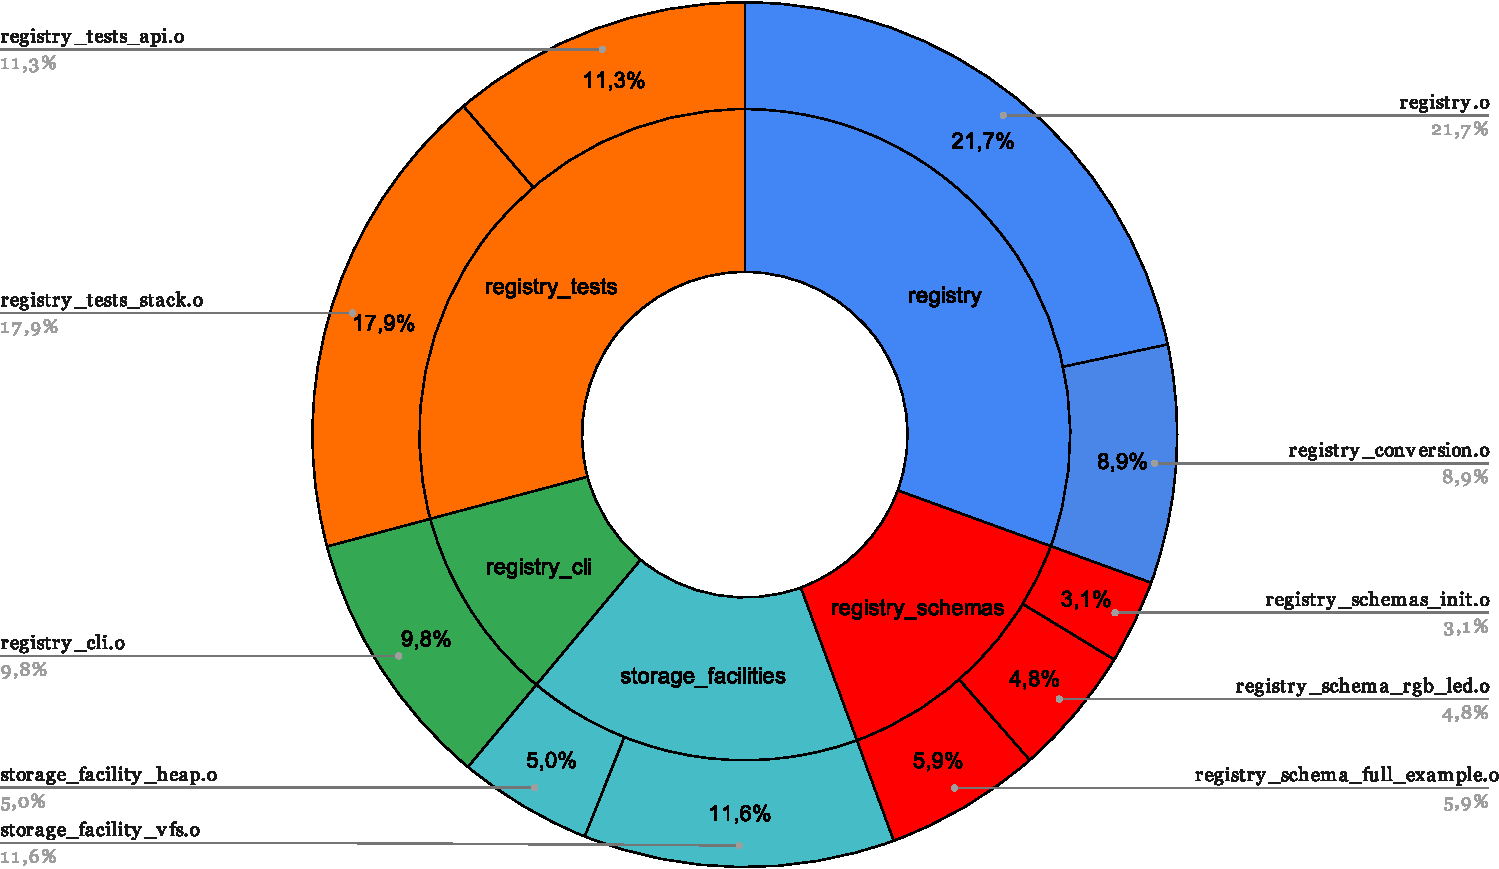
\includegraphics[width=\textwidth]{evaluation_rom_pie_chart}
    \caption{\nameref{sec:design:riot_registry} ROM usage per module (inner circle) and per object file (outer circle).}
    \label{fig:evaluation:rom_usage_per_module}
\end{figure}

\subsubsection{Discussion}

The more fine-grained measurements are helpful because the ``registry\_schemas'' and ``registry\_storage\_facilites'' modules allow to enable and disable each \gls{ac:cs} and \gls{ac:sf} implementation separately.
This way a lot of ROM overhead can be avoided by only enabling what is needed and these measurements show about how much can be saved.

It should also be noted that the ``registry\_tests'' module is usually not enabled when using the \nameref{sec:design:riot_registry}.